% !TEX encoding = UTF-8 Unicode
%!TEX TS-program = xelatex

\documentclass[12pt]{extarticle}
% extarticle is like article but can handle 8pt, 9pt, 10pt, 11pt, 12pt, 14pt, 17pt, and 20pt text

\def \ititle {Origins of Mind}
 
\def \isubtitle {Lecture 08}
 
\def \iauthor {Stephen A. Butterfill}
\def \iemail{s.butterfill@warwick.ac.uk}
\date{}

%for strikethrough
\usepackage[normalem]{ulem}

\usepackage{pdfpages}


\input{$HOME/Documents/submissions/preamble_steve_handout}

%logic symbol \leftmodels
\usepackage{MnSymbol}

%\bibpunct{}{}{,}{s}{}{,}  %use superscript TICS style bib
%remove hanging indent for TICS style bib
%TODO doesnt work
\setlength{\bibhang}{0em}
%\setlength{\bibsep}{0.5em}


%itemize bullet should be dash
\renewcommand{\labelitemi}{$-$}

\begin{document}

%\raggedcolumns

\begin{multicols*}{3}

\setlength\footnotesep{1em}


\bibliographystyle{newapa} %apalike

%\maketitle
%\tableofcontents




%--------------- 
%--- start paste

\def \ititle {Logic I}
 
\def \isubtitle {Lecture 12}
 
\begin{center}
 
{\Large
 
\textbf{\ititle}: \isubtitle
 
}
 
 
 
\iemail %
 
\end{center}
 
Readings refer to sections of the course textbook, \emph{Language, Proof and Logic}.
 
 
 
\section{Relations: Reflexive, Symmetric}
 
\emph{Reading:} §15.1
 
A \emph{reflexive} relation is one that everything bears to itself. (E.g. everything is the SameShape as itself. E.g. of non-reflexive: not everything is LeftOf itself).
 
A \emph{symmetric} relation is one such that if x bears it to y, then y bears it to x. (E.g. Adjacent(x,y) is symmetric, LeftOf(x,y) is not symmetric.)
 
 
 
\section{Relations: Transitivity}
 
\emph{Reading:} §15.1
 
A \emph{transitive} relation is one such that if x bears it to y and y bears it to z then x bears it to z. (E.g. LeftOf is transitive; NotAdjacent is not transitive.)
 
\begin{minipage}{\columnwidth}
 
If NotAdjacent were transitive, the following argument would be logically valid:
 
\begin{center}
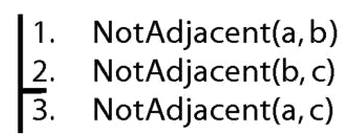
\includegraphics[scale=0.3]{img/unit_125_argument.png}
\end{center}
\end{minipage}
 
\begin{minipage}{\columnwidth}
 
A counterexample to this argument:
 
\begin{center}
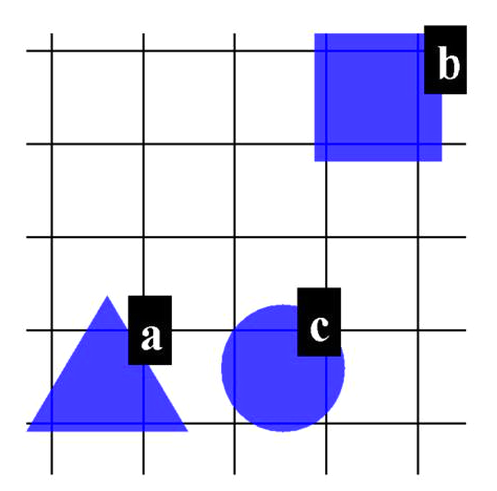
\includegraphics[scale=0.3]{img/unit_125_counterexample.png}
\end{center}
\end{minipage}
 
 
 
\section{Relations: Some Examples}
 
\emph{Reading:} §15.1
 
\begin{center}
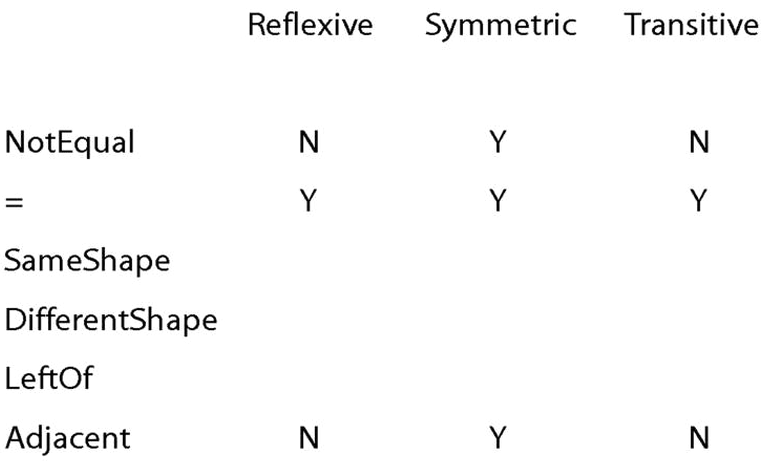
\includegraphics[scale=0.3]{img/unit_128_fig.png}
\end{center}
Artificial relations ...
 
EqualToOrLeftOf(x, y) iff
 
\hspace{3mm} x = y or LeftOf(x, y)
 
EqualToOrAdjacent(x, y) iff
 
\hspace{3mm} x=y or Adjacent(x, y)
 
JohnOrAyesha(x, y) iff
 
\hspace{3mm} x = John and y = Ayesha
 
\hspace{3mm} or x = Ayesha and y = John
 
JohnToAyesha(x, y) iff
 
\hspace{3mm} x = John and y = Ayesha
 
 
 
\section{Expressing Relations with Quantifiers}
 
\emph{Reading:} §15.1
 
\begin{minipage}{\columnwidth}
 
A \emph{reflexive} relation is one that everything bears to itself. (E.g. SameShape)
 
reflexive: ∀x R(x,x)
 
\begin{center}
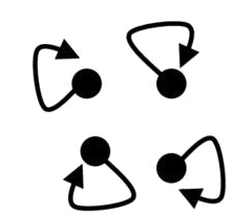
\includegraphics[scale=0.3]{img/reflexive.png}
\end{center}
\end{minipage}
 
\begin{minipage}{\columnwidth}
 
A \emph{symmetric} relation is one such that if x bears it to y, then y bears it to x. (E.g. Adjacent(x,y))
 
symmetric: ∀x∀y ( R(x,y) → R(y,x) )
 
\begin{center}
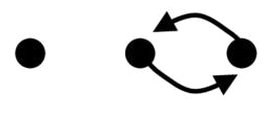
\includegraphics[scale=0.3]{img/symmetric.png}
\end{center}
\end{minipage}
 
\begin{minipage}{\columnwidth}
 
A \emph{transitive} relation is one such that if x bears it to y and y bears it to z then x bears it to z. (E.g. LeftOf is transitive; DifferentShape is not transitive)
 
transitive: ∀x∀y∀z ( ( R(x,y) ∧ R(y,z) ) → R(x,z) )
 
\begin{center}
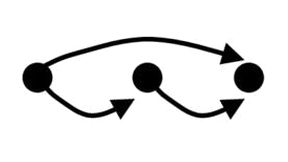
\includegraphics[scale=0.3]{img/transitive.png}
\end{center}
\end{minipage}
 
 
 
\section{Negating Identity}
 
\begin{center}
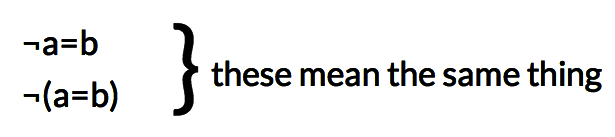
\includegraphics[scale=0.3]{img/unit_323.png}
\end{center}
 
 
\section{Expressing Counterexamples Formally}
 
\emph{Reading:} §15.1
 
Give a counterexample to this argument:
 
\begin{center}
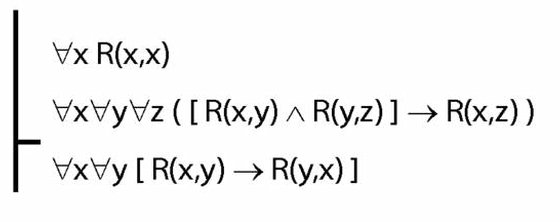
\includegraphics[scale=0.3]{img/unit_583_argument.png}
\end{center}
Informally:
 
\begin{center}
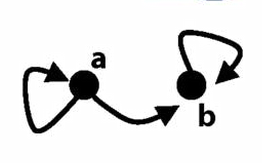
\includegraphics[scale=0.3]{img/unit_583_counterexample.png}
\end{center}
Formally:
 
\hspace{3mm} Domain: \{a, b\}
 
\hspace{3mm} R: \{<a,a>, <a,b>, <b,b>\}
 
 
 
\section{Proof Example: A∧B therefore ¬(¬A∨¬B).}
 
\begin{center}
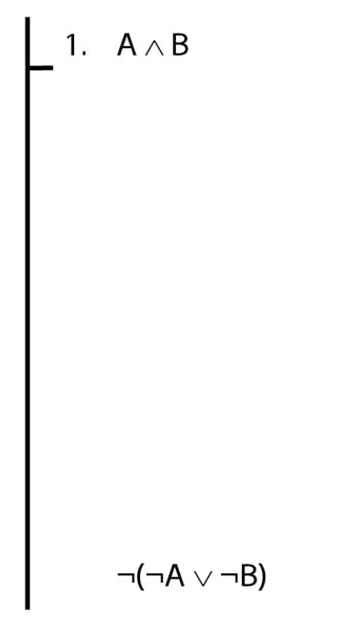
\includegraphics[scale=0.3]{img/unit_822_proof.png}
\end{center}
 
 
\section{Proof Example: P therefore ¬¬P.}
 
\begin{center}
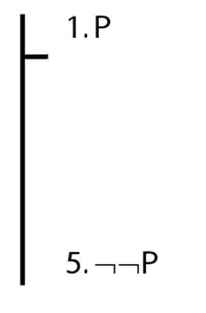
\includegraphics[scale=0.3]{img/unit_823_proof.png}
\end{center}
 
 
\section{Proof Example: S∨(Q∧R) therefore S∨Q.}
 
\begin{center}
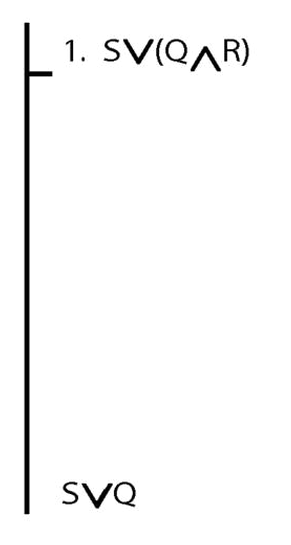
\includegraphics[scale=0.3]{img/unit_824_proof.png}
\end{center}
\vfill

%--- end paste
%--------------- 
 


\end{multicols*}

\end{document}